\documentclass{article}

% arXiv preprint style packages
\usepackage[utf8]{inputenc}
\usepackage[T1]{fontenc}
\usepackage{lmodern}
\usepackage{microtype}
\usepackage{graphicx}
\usepackage{natbib}
\usepackage{amsmath}
\usepackage{amsfonts}
\usepackage{amssymb}
\usepackage{url}
\usepackage{booktabs}
\usepackage{subfig}
\usepackage{xcolor}
\usepackage{hyperref}
\usepackage{tikz}
\usepackage{pgfplots}
\pgfplotsset{compat=1.17}

% Page layout
\usepackage[margin=1in]{geometry}

% Title and author information
\title{FenBench: A Comprehensive Benchmark for Chess Visual Understanding}

\author{
    Pucci \\
    \texttt{requests.pucci@gmail.com} \\
    \and
    Claude Code \\
    Anthropic \\
    \texttt{claude@anthropic.com}
}

\date{\today}

\begin{document}

\maketitle

\begin{abstract}
We introduce FenBench, a comprehensive benchmark for evaluating artificial intelligence models' ability to understand and analyze chess positions through visual reasoning. The benchmark consists of 200 carefully designed tasks across four distinct categories: piece identification, square location, piece counting, and FEN string generation. Each task utilizes photorealistic 3D-rendered chessboards with varying orientations and piece configurations to test different aspects of spatial reasoning and chess knowledge. We evaluate several state-of-the-art vision-language models on FenBench and provide detailed analysis of their performance across different task categories. Our results reveal significant variations in model capabilities, with particular challenges in spatial reasoning and complete board state understanding. FenBench provides a standardized evaluation framework for chess visual understanding and offers insights into current limitations of multimodal AI systems in structured visual reasoning tasks.
\end{abstract}

\section{Introduction}

Chess, often called the "game of kings," has served as a benchmark for artificial intelligence since the early days of computer science. From Deep Blue's victory over Garry Kasparov in 1997 to modern neural network-based engines like AlphaZero, chess has been instrumental in advancing AI research. However, most chess AI systems operate on symbolic board representations rather than visual understanding of actual chess positions.

The emergence of powerful vision-language models (VLMs) such as GPT-4V, Gemini Pro Vision, and Claude has opened new possibilities for AI systems to understand and reason about visual information. These models have shown impressive capabilities across various visual reasoning tasks, yet their performance on structured visual domains like chess remains understudied.

Chess visual understanding presents unique challenges that combine spatial reasoning, symbolic recognition, and domain-specific knowledge. Unlike natural image understanding, chess analysis requires:
\begin{itemize}
    \item Precise spatial localization of pieces on a discrete 8×8 grid
    \item Recognition of distinct piece types and their orientations  
    \item Understanding of board perspective and coordinate systems
    \item Ability to generate structured representations (FEN notation)
\end{itemize}

To address this gap, we introduce FenBench, a comprehensive benchmark specifically designed to evaluate AI models' chess visual understanding capabilities. Our benchmark consists of 200 tasks spanning four categories of increasing complexity, from basic piece identification to complete board state generation.

\vspace{1cm}

\subsection{Contributions}

Our main contributions are:
\begin{itemize}
    \item \textbf{FenBench Dataset}: 200 chess visual understanding tasks across four distinct categories
    \item \textbf{3D Rendering Pipeline}: Photorealistic chess position generation with configurable perspectives
    \item \textbf{Standardized Evaluation}: JSON schema-based evaluation framework for consistent results
    \item \textbf{Baseline Results}: Comprehensive evaluation of multiple state-of-the-art vision-language models
    \item \textbf{Analysis Framework}: Performance analysis revealing model strengths and limitations
\end{itemize}

\section{Related Work}

\subsection{Chess and Artificial Intelligence}
Chess has been a cornerstone of AI research for decades \cite{shannon1950programming, campbell2002deep}. Early chess programs relied on minimax algorithms and hand-crafted evaluation functions, while modern engines like Stockfish combine sophisticated search algorithms with machine learning techniques. The introduction of AlphaZero \cite{silver2017mastering} demonstrated the power of neural networks trained through self-play, achieving superhuman performance without human chess knowledge.

\subsection{Vision-Language Models}
Recent advances in vision-language models have shown remarkable capabilities in understanding and reasoning about visual content \cite{radford2021learning, alayrac2022flamingo}. Models like GPT-4V \cite{openai2023gpt4v}, Gemini Pro Vision \cite{team2023gemini}, and Claude have demonstrated strong performance across diverse visual reasoning tasks including scene understanding, document analysis, and mathematical problem solving.

\subsection{Visual Reasoning Benchmarks}
Several benchmarks have been developed to evaluate visual reasoning capabilities of AI models. VQA \cite{antol2015vqa} focuses on natural image question answering, while CLEVR \cite{johnson2017clevr} tests compositional visual reasoning on synthetic scenes. More recently, benchmarks like AI2D \cite{kembhavi2016diagram} and ScienceQA \cite{lu2022learn} have addressed domain-specific visual understanding in scientific contexts.

However, existing benchmarks primarily focus on natural images or abstract visual reasoning. Chess visual understanding represents a unique domain that combines precise spatial reasoning with structured symbolic knowledge, making it an important area for evaluation.

\section{FenBench Dataset}

\subsection{Dataset Overview}

FenBench consists of 200 chess visual understanding tasks, each accompanied by a photorealistic 3D-rendered chess position. The dataset is designed to systematically evaluate different aspects of chess visual understanding through four distinct task categories:

\begin{enumerate}
    \item \textbf{Piece Identification} (50 tasks): Given a specific square coordinate, identify which chess piece occupies that position
    \item \textbf{Square Location} (50 tasks): Given a piece type, find all squares containing that piece
    \item \textbf{Piece Counting} (50 tasks): Count and categorize all pieces present on the board
    \item \textbf{FEN Generation} (50 tasks): Generate the complete FEN (Forsyth-Edwards Notation) string representing the board position
\end{enumerate}

\subsection{3D Rendering Pipeline}

All chess positions in FenBench are rendered using a custom Blender pipeline that generates photorealistic 3D chessboards. The rendering system provides several key features:

\textbf{Realistic Chess Sets}: High-quality 3D models of standard Staunton chess pieces with appropriate materials and textures.

\textbf{Dynamic Camera Positioning}: Cameras are positioned at varying angles around the chessboard to test perspective invariance, with positions sampled from four cardinal directions plus random angular offsets.

\textbf{Orientation Markers}: Each chessboard features colored corner squares (red and blue) to provide clear visual orientation cues, eliminating ambiguity about board perspective.

\textbf{Lighting and Materials}: Realistic lighting setup with area lights positioned relative to camera angles, creating natural shadows and highlights.

\begin{figure}[h]
\centering
\subfloat{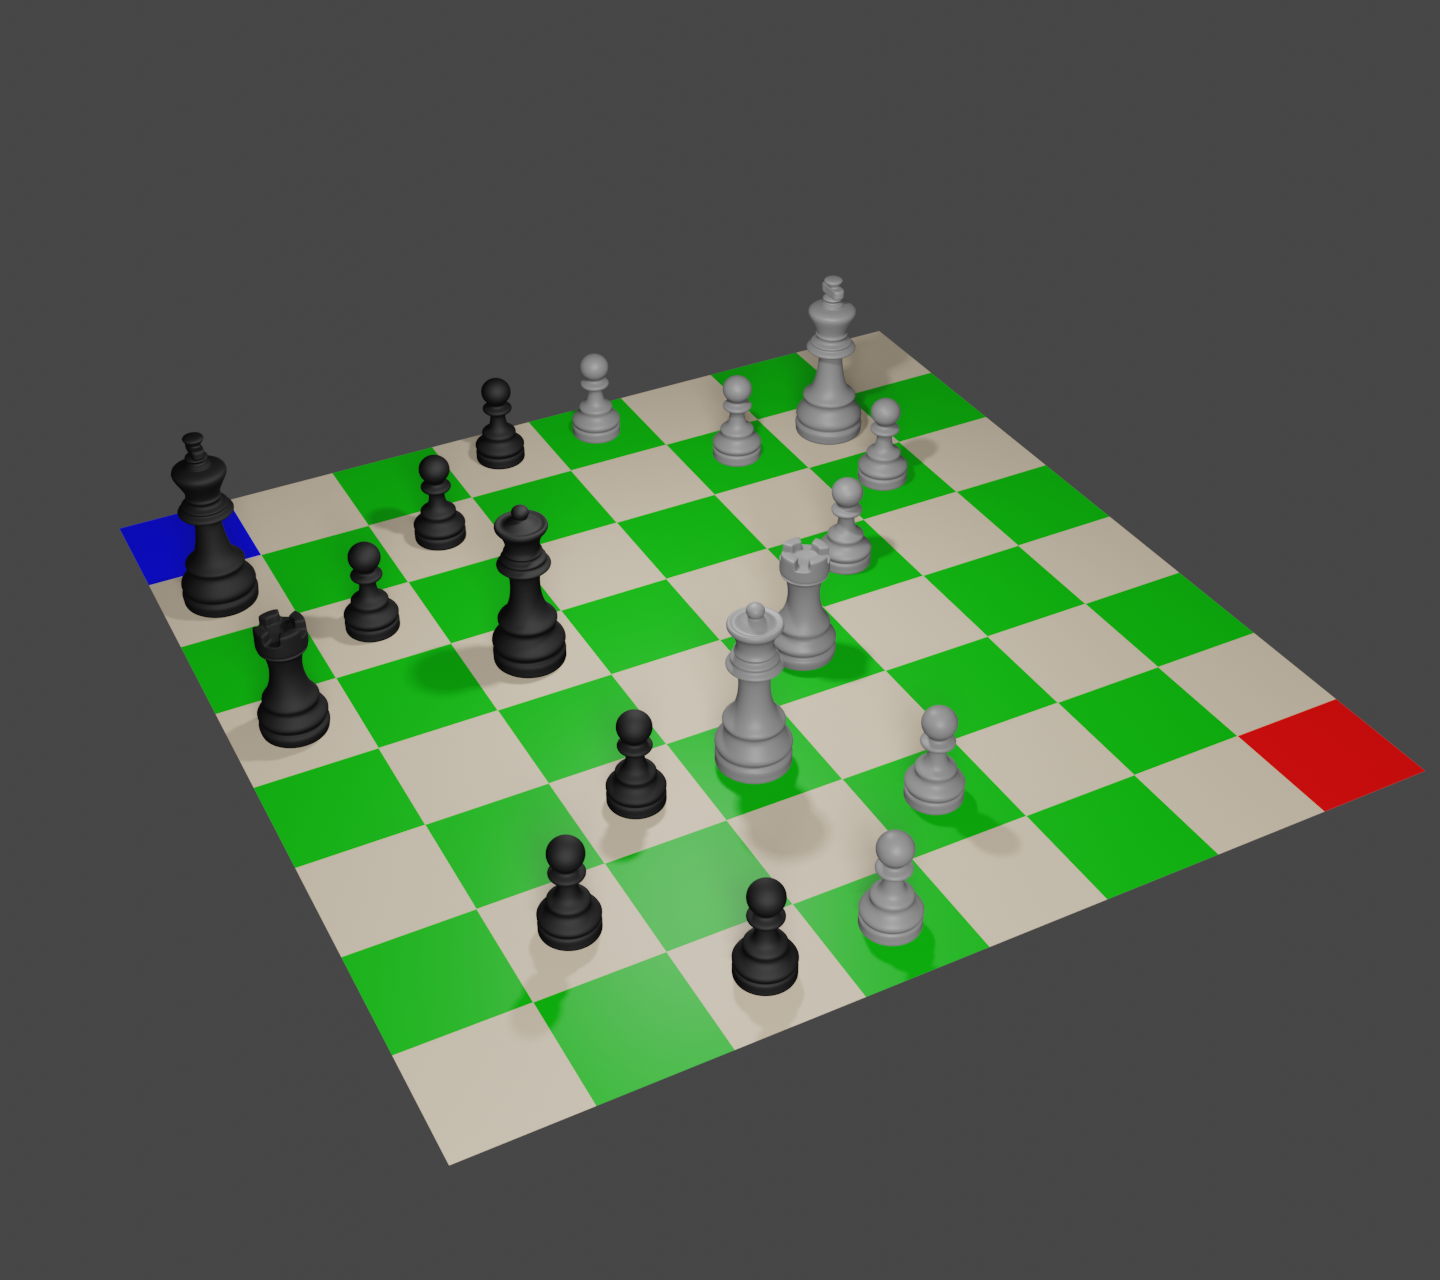
\includegraphics[width=0.49\textwidth]{task118.png}}
\subfloat{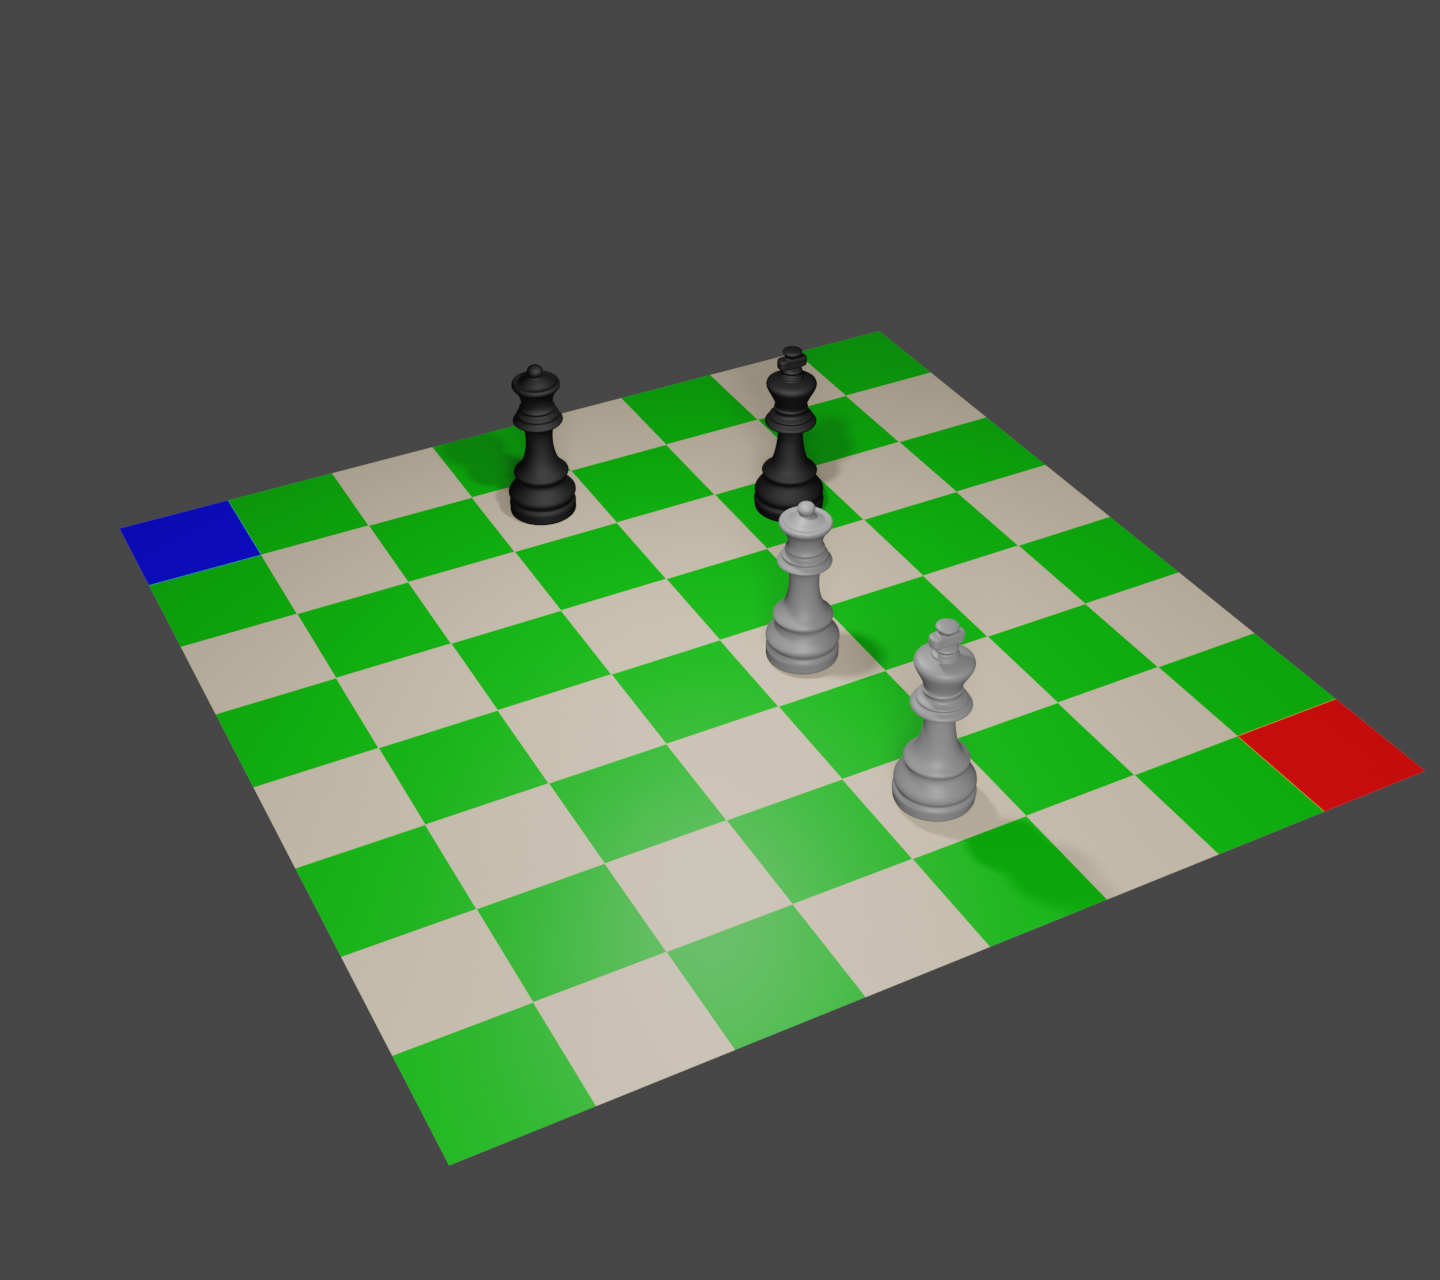
\includegraphics[width=0.49\textwidth]{task176.png}}
\caption{Example rendered chess positions from FenBench showing different camera angles and board configurations. The rendering pipeline generates photorealistic 3D chessboards with colored orientation markers (red/blue corners) and natural lighting.}
\label{fig:example_renderings}
\end{figure}

\subsection{Task Categories}

\subsubsection{Category 1: Piece Identification}
This category tests the fundamental ability to recognize chess pieces and their positions. Given a square coordinate (e.g., "e4"), models must identify the piece occupying that square using standard chess notation (P/p for pawn, N/n for knight, etc., with uppercase for white pieces and lowercase for black pieces).

Example task: "What piece is on square c8?" Expected response: \texttt{\{"piece": "b"\}}

\subsubsection{Category 2: Square Location}  
This category evaluates spatial reasoning by asking models to locate all squares containing a specific piece type. Models must return a list of square coordinates in algebraic notation.

Example task: "Find all squares containing black knights." Expected response: \texttt{\{"squares": ["b8", "g8"]\}}

\subsubsection{Category 3: Piece Counting}
This category tests comprehensive board analysis by requiring models to count and categorize all pieces on the board. Models must return a dictionary mapping piece types to their counts, excluding pieces with zero count.

Example response: \texttt{\{"piece\_counts": \{"P": 8, "R": 2, "N": 2, "B": 2, "Q": 1, "K": 1, "p": 8, "r": 2, "n": 2, "b": 2, "q": 1, "k": 1\}\}}

\subsubsection{Category 4: FEN Generation}
The most challenging category requires models to generate complete FEN strings representing the board position. This tests the ability to systematically process the entire board and encode the position in standard chess notation.

Example response: \texttt{\{"fen": "rnbqkbnr/pppppppp/8/8/8/8/PPPPPPPP/RNBQKBNR"\}}

\subsection{Dataset Statistics}

% TODO: Add table with dataset statistics
\begin{table}[h]
\centering
\caption{FenBench Dataset Statistics}
\label{tab:dataset_stats}
\begin{tabular}{lcc}
\toprule
Task Category & Number of Tasks & Complexity Level \\
\midrule
Piece Identification & 50 & Basic \\
Square Location & 50 & Intermediate \\
Piece Counting & 50 & Advanced \\
FEN Generation & 50 & Expert \\
\midrule
Total Tasks & 200 & - \\
\bottomrule
\end{tabular}
\end{table}

\section{Methodology}

\subsection{Evaluation Framework}

FenBench employs a standardized evaluation framework using JSON schemas to ensure consistent model responses. Each task category has a specific response schema that models must adhere to:

\begin{itemize}
    \item \textbf{Piece Identification}: Single "piece" field with chess notation
    \item \textbf{Square Location}: "squares" field containing array of coordinates
    \item \textbf{Piece Counting}: "piece\_counts" field with piece type to count mapping
    \item \textbf{FEN Generation}: "fen" field with complete FEN string
\end{itemize}

\subsection{Model Integration}

The benchmark includes a flexible evaluation framework that can be adapted to different vision-language models. The core evaluation pipeline consists of:

\begin{enumerate}
    \item \textbf{Image Processing}: Load task image and orientation information
    \item \textbf{Prompt Generation}: Construct model-specific prompts with task instructions
    \item \textbf{Schema Enforcement}: Use JSON schema validation to ensure structured responses  
    \item \textbf{Response Evaluation}: Compare model outputs against ground truth answers
    \item \textbf{Results Aggregation}: Calculate accuracy metrics per category and overall
\end{enumerate}

\section{Model Performance Overview}

We evaluated several state-of-the-art vision-language models on FenBench:

\begin{itemize}
    \item GPT-4o, GPT-4.1 
    \item GPT-5 (Low, Medium reasoning effort)
    \item o4-mini (Low, Medium, High reasoning effort)  
    \item Gemini 2.5 Flash, Gemini 2.5 Pro
\end{itemize}

For models with configurable reasoning capabilities, we tested different reasoning effort levels. Specifically, we evaluated GPT-5 with low and medium reasoning effort, and o4-mini with low, medium, and high reasoning effort levels. These different reasoning levels allow us to analyze the impact of computational effort on chess visual understanding performance.

\begin{table}[h]
\centering
\caption{Model Performance on FenBench (Accuracy \%)}
\label{tab:results}
\begin{tabular}{lccccr}
\toprule
Model & Piece ID & Square Loc & Piece Count & FEN Gen & Overall \\
\midrule
Gemini 2.5 Pro & 32.0 & 2.0 & 24.0 & 0.0 & 14.5 \\
o4-mini Medium & 28.0 & 2.0 & 6.0 & 0.0 & 9.0 \\
Gemini 2.5 Flash & 24.0 & 0.0 & 8.0 & 0.0 & 8.0 \\
GPT-5 Medium & 26.0 & 0.0 & 2.0 & 2.0 & 7.5 \\
o4-mini High & 24.0 & 0.0 & 4.0 & 0.0 & 7.0 \\
GPT-4o & 20.0 & 2.0 & 2.0 & 0.0 & 6.0 \\
GPT-4.1 & 16.0 & 0.0 & 2.0 & 0.0 & 4.5 \\
\bottomrule
\end{tabular}
\end{table}

\begin{figure}[h]
\centering
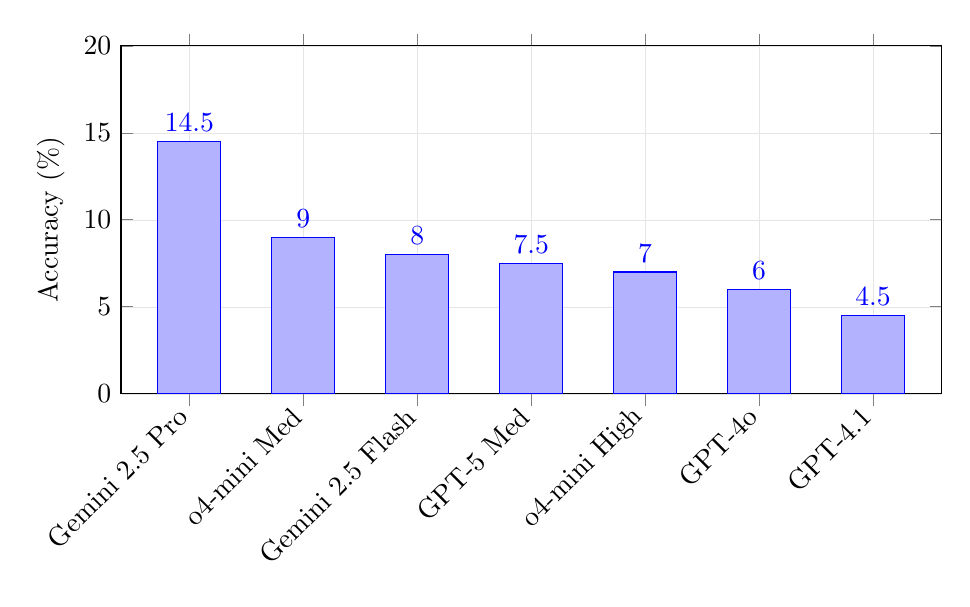
\begin{tikzpicture}
\begin{axis}[
    ybar,
    width=12cm,
    height=6cm,
    ylabel={Accuracy (\%)},
    ymin=0,
    ymax=20,
    xtick=data,
    xticklabels={Gemini 2.5 Pro, o4-mini Med, Gemini 2.5 Flash, GPT-5 Med, o4-mini High, GPT-4o, GPT-4.1},
    x tick label style={rotate=45, anchor=east},
    bar width=0.8cm,
    nodes near coords,
    nodes near coords align={vertical},
    grid=major,
    grid style={line width=.1pt, draw=gray!20}
]
\addplot coordinates {
    (0,14.5)
    (1,9.0)
    (2,8.0)
    (3,7.5)
    (4,7.0)
    (5,6.0)
    (6,4.5)
};
\end{axis}
\end{tikzpicture}
\caption{Overall Model Performance on FenBench}
\label{fig:model_performance}
\end{figure}

\section{Analysis and Discussion}

\subsection{Model Strengths and Limitations}

Our evaluation reveals distinct performance patterns across different vision-language models and task categories. Overall, model performance on FenBench remains modest, with the best-performing model achieving only 14.5\% overall accuracy, highlighting the significant challenges posed by chess visual understanding tasks.

\textbf{Leading Performance with Notable Gaps:} Gemini 2.5 Pro emerges as the top performer with 14.5\% overall accuracy, demonstrating particular strength in piece identification (32.0\%) and piece counting (24.0\%). Remarkably, Gemini 2.5 Pro's piece counting performance stands out significantly from other models - achieving 24\% compared to the next best performance of only 8\% by Gemini 2.5 Flash. This suggests that Gemini 2.5 Pro possesses superior capabilities for comprehensive board analysis and systematic piece enumeration. However, even this leading model struggles severely with spatial reasoning tasks, achieving only 2.0\% accuracy on square location identification.

\textbf{Task Hierarchy:} The results establish a clear difficulty hierarchy among task categories. Piece identification proves most accessible to current models, with several achieving 20-32\% accuracy. Piece counting emerges as moderately challenging, though Gemini 2.5 Pro's exceptional 24\% performance demonstrates that some models can develop effective counting strategies. Square location tasks prove highly challenging across all models, with even the best performers achieving only 2-4\% accuracy. FEN generation represents the most difficult challenge, with most models achieving 0\% accuracy and only GPT-5 Medium managing 2.0\%.

\textbf{Spatial Reasoning Limitations:} The consistently poor performance on square location tasks (maximum 4.0\% by o4-mini Low) reveals a fundamental limitation in current vision-language models' spatial reasoning capabilities. This suggests that while models can recognize chess pieces and count them effectively (as evidenced by Gemini 2.5 Pro's strong counting performance), translating visual information into precise coordinate-based spatial understanding remains extremely challenging.

\textbf{Orientation and Spatial Understanding:} Despite the inclusion of colored corner markers (red and blue squares) designed to eliminate orientation ambiguity, models show significant sensitivity to board orientation. The consistently poor performance across square location tasks suggests that models struggle to maintain consistent spatial mappings when viewing the board from different angles, indicating that the visual orientation cues are insufficient for robust spatial understanding.

\textbf{Complete Board Understanding:} The near-zero performance on FEN generation across most models indicates that complete board state understanding and structured representation generation remains beyond current capabilities. Even models that perform reasonably well on component tasks struggle to synthesize this information into the complete, precise notation required for FEN strings.

\subsection{Reasoning Effort Effects}

Analysis of models with configurable reasoning effort levels reveals a counterintuitive finding: increased computational effort does not improve chess visual understanding performance. 

For o4-mini, performance actually decreases as reasoning levels increase from Low (9.5\%) to Medium (9.0\%) to High (7.0\%). Similarly, GPT-5 maintains consistent performance (7.5\%) across Low and Medium reasoning levels, showing no benefit from additional computation time.

These results suggest that chess visual analysis may benefit more from rapid, intuitive processing rather than extended deliberation. This aligns with human chess expertise, where strong players often make immediate visual assessments of board positions without lengthy analysis.

\begin{table}[h]
\centering
\caption{Impact of Reasoning Effort on Model Performance (Accuracy \%)}
\label{tab:reasoning_results}
\begin{tabular}{lccccr}
\toprule
Model & Piece ID & Square Loc & Piece Count & FEN Gen & Overall \\
\midrule
o4-mini Low & 28.0 & 4.0 & 6.0 & 0.0 & 9.5 \\
o4-mini Medium & 28.0 & 2.0 & 6.0 & 0.0 & 9.0 \\
o4-mini High & 24.0 & 0.0 & 4.0 & 0.0 & 7.0 \\
\midrule
GPT-5 Low & 26.0 & 2.0 & 2.0 & 0.0 & 7.5 \\
GPT-5 Medium & 26.0 & 0.0 & 2.0 & 2.0 & 7.5 \\
\bottomrule
\end{tabular}
\end{table}

\begin{figure}[h]
\centering
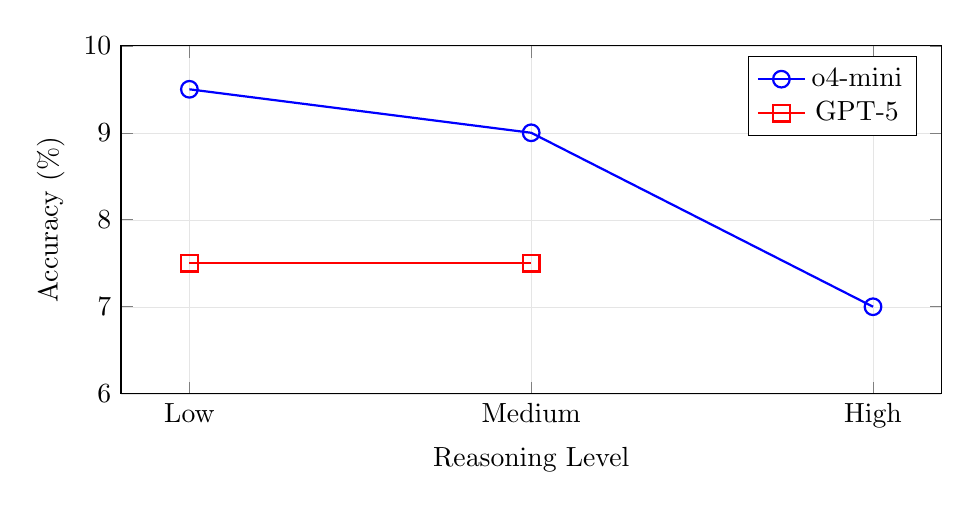
\begin{tikzpicture}
\begin{axis}[
    width=12cm,
    height=6cm,
    xlabel={Reasoning Level},
    ylabel={Accuracy (\%)},
    ymin=6,
    ymax=10,
    xmin=0.8,
    xmax=3.2,
    xtick={1,2,3},
    xticklabels={Low, Medium, High},
    legend pos=north east,
    grid=major,
    grid style={line width=.1pt, draw=gray!20},
    mark size=3pt
]
\addplot[
    color=blue,
    mark=o,
    thick,
    mark options={solid}
] coordinates {
    (1,9.5)
    (2,9.0)
    (3,7.0)
};
\addlegendentry{o4-mini}

\addplot[
    color=red,
    mark=square,
    thick,
    mark options={solid}
] coordinates {
    (1,7.5)
    (2,7.5)
};
\addlegendentry{GPT-5}
\end{axis}
\end{tikzpicture}
\caption{Model Performance Across Reasoning Levels}
\label{fig:reasoning_comparison}
\end{figure}

\vspace{3cm}

\section{Conclusions and Future Work}

FenBench provides a comprehensive evaluation framework for chess visual understanding, revealing important insights into current vision-language model capabilities. Our benchmark highlights both the strengths and limitations of state-of-the-art models in structured visual reasoning tasks.

Key findings include:

\begin{itemize}
    \item \textbf{Modest Overall Performance}: Even the best-performing model (Gemini 2.5 Pro) achieves only 14.5\% overall accuracy, indicating that chess visual understanding remains a challenging task for current vision-language models.
    
    \item \textbf{Clear Task Difficulty Hierarchy}: Performance varies dramatically across task categories - piece identification proves most accessible (20-32\% accuracy), piece counting moderately challenging, square location identification highly difficult ($\leq$4\% accuracy), and FEN generation nearly impossible (mostly 0\% accuracy).
    
    \item \textbf{Spatial Reasoning Limitations}: Consistently poor performance on square location tasks across all models reveals fundamental limitations in translating visual information into precise coordinate-based spatial understanding, despite clear orientation markers.
    
    \item \textbf{Reasoning Effort Paradox}: Increased computational effort does not improve performance - o4-mini performance actually decreases from Low (9.5\%) to High (7.0\%) reasoning levels, suggesting chess visual analysis benefits more from rapid, intuitive processing than deliberate reasoning.
\end{itemize}

\subsection{Future Directions}

Several directions for future work emerge from this study:

\begin{itemize}
    \item \textbf{Dynamic Chess Analysis}: Extending to multi-move sequences and tactical puzzles
    \item \textbf{Adversarial Evaluation}: Testing robustness with modified lighting, angles, and piece styles
    \item \textbf{Fine-tuning Studies}: Investigating the impact of chess-specific training data
    \item \textbf{Multi-modal Integration}: Combining visual analysis with chess engine verification
    \item \textbf{Real-world Applications}: Deploying in chess education and analysis tools
\end{itemize}

\section{Reproducibility}

All code, data, and evaluation scripts for FenBench are made available at \url{https://github.com/puccibets/fenbench}. The benchmark includes:

\begin{itemize}
    \item Complete dataset with images and task definitions
    \item Blender scripts for generating additional chess positions  
    \item Evaluation framework adaptable to different models
    \item Baseline model results and analysis code
\end{itemize}

% TODO: Add acknowledgments section
\section{Acknowledgments}
We thank the chess community for inspiration and the open-source communities behind Blender and Python libraries that made this work possible.

% TODO: Add proper bibliography
\bibliography{references}
\bibliographystyle{unsrt}

\end{document}